\section{Phoneme-Based Informational Masking}

\begin{figure}[t]
    \centering
    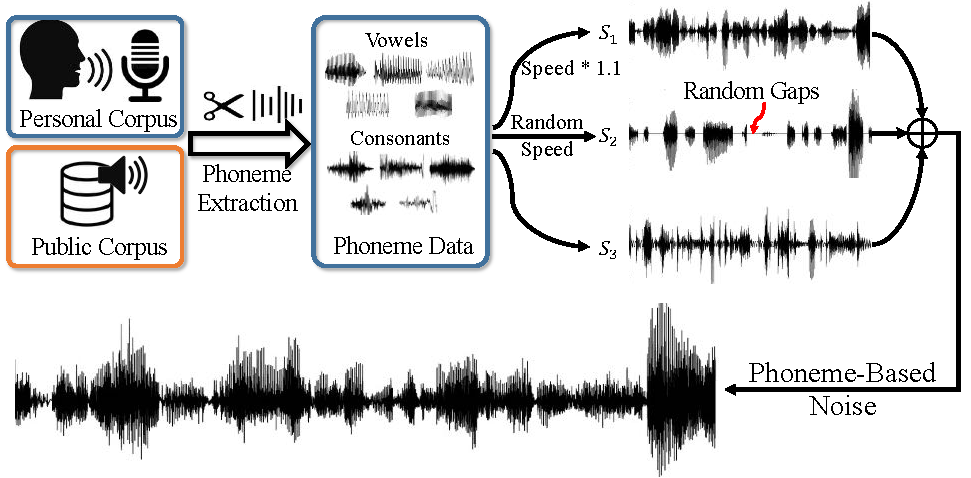
\includegraphics[width=\linewidth]{images/noise_design.pdf}
    \caption{Generation of phoneme-based noise. }
    \label{fig:full_noise_design}
    \vspace{-6mm}
\end{figure}

\label{sec:noise_design}
\subsection{Key Insight}
The main goal of this paper is jamming microphones in the environment by transmitting noise to make the recordings unrecognizable to both human and ASR systems. The success of jamming ASR systems mainly relies on the noise's robustness against speech enhancement methods, while the success of jamming the human auditory system mainly relies on the two masking effects: informational masking and energetic masking. The effectiveness of energetic masking mainly depends on the relative energy of the noise to the target signal, while for the latter, it mainly depends on the content of the noise~\cite{brungart_informational_2001,leek_informational_1991, festen_effects_1990}. Existing works \cite{backdoor, patronus, CHI} focus on utilizing energetic masking, which leads to a high demand for energy and is not suitable in the ultrasonic transmission scenario.

In this paper, our key insight is exploiting the informational masking effect to form noise. Previous studies have shown that when presented with noises, the differences in phonetical properties such as fundamental frequency (F0) between the noise and the target speech will assist listeners to filter out the noise and understand the target speech signal\cite{brungart_informational_2001}. Therefore, we first construct noise that has similar F0 to the target speech signal. Additionally, through experiments we find that the difference in speech rate between the noise and the speech also affects the effectiveness of informational masking, which inspires us to treat speech rate as another factor in our phoneme-based noise design.

\subsection{Noise Design}
\label{subsec:noise_design}

As shown in Figure \ref{fig:full_noise_design}, our phoneme-based noise consists of three phoneme sequences: $S_1$, $S_2$, and $S_3$. $S_1$ is a sequence of random vowels without gaps in between, and it is accelerated by a preset parameter to include more vowels per unit time for better jamming effectiveness, and the parameter is set to 1.1 according to our experiments. The reason we choose vowels is that compared to consonants, vowels make up most of the energy in speech signals. Because the difference in phonetical properties such as fundamental frequency (F0) between the speech signal and the noise will assist listeners in separating the noise, we extract the phoneme data from the target people's speech materials to minimize such difference. Simple concatenation of the phoneme data will cause discontinuity at phoneme boundaries. To smooth the connected phoneme data, we apply a hamming window with a length of 25ms at the juncture between phonemes. Without special mention, this smoothing method is also applied to the following sequences that make up our noises.

Then we consider narrowing down the speech rate gap between the noise and the target signal. Since the target signal's speech rate is unknown, we add another vowel sequence $S_2$ with random speech rate. Different from $S_1$, there are gaps of random length between the vowels in $S_2$. Each vowel is accelerated or decelerated with a randomly chosen speed factor that follows a uniform distribution $U(0.3, 1.8)$ which is chosen according to our experimental results. In addition to making the rate more similar to the target signal, $S_2$ also makes the noise more varied and shows less constant patterns, which helps with the robustness against noise reduction methods.

Apart from vowels, we add a consonant sequence $S_3$ to increase the diversity of noise. As the difference in consonants between different people is much smaller than that in vowels, we utilize the consonant data from a public speech corpus (LibriSpeech \cite{LibriSpeech}). Then we connect these consonants without gaps to form $S_3$.

Our noise is the superposition of the above three phoneme sequences. To demonstrate the feasibility, we test its robustness against the built-in noise reduction in a smartphone. We play voices along with various types of noise and record the signal with the phone. The results in Figure~\ref{fig:test_denoise_in_noise_design} show that our noise is robust against the built-in noise reduction while the others are suppressed significantly.

\begin{figure}[!t]
    \centering
    \begin{subfigure}[b]{0.49\columnwidth}
        \centering
        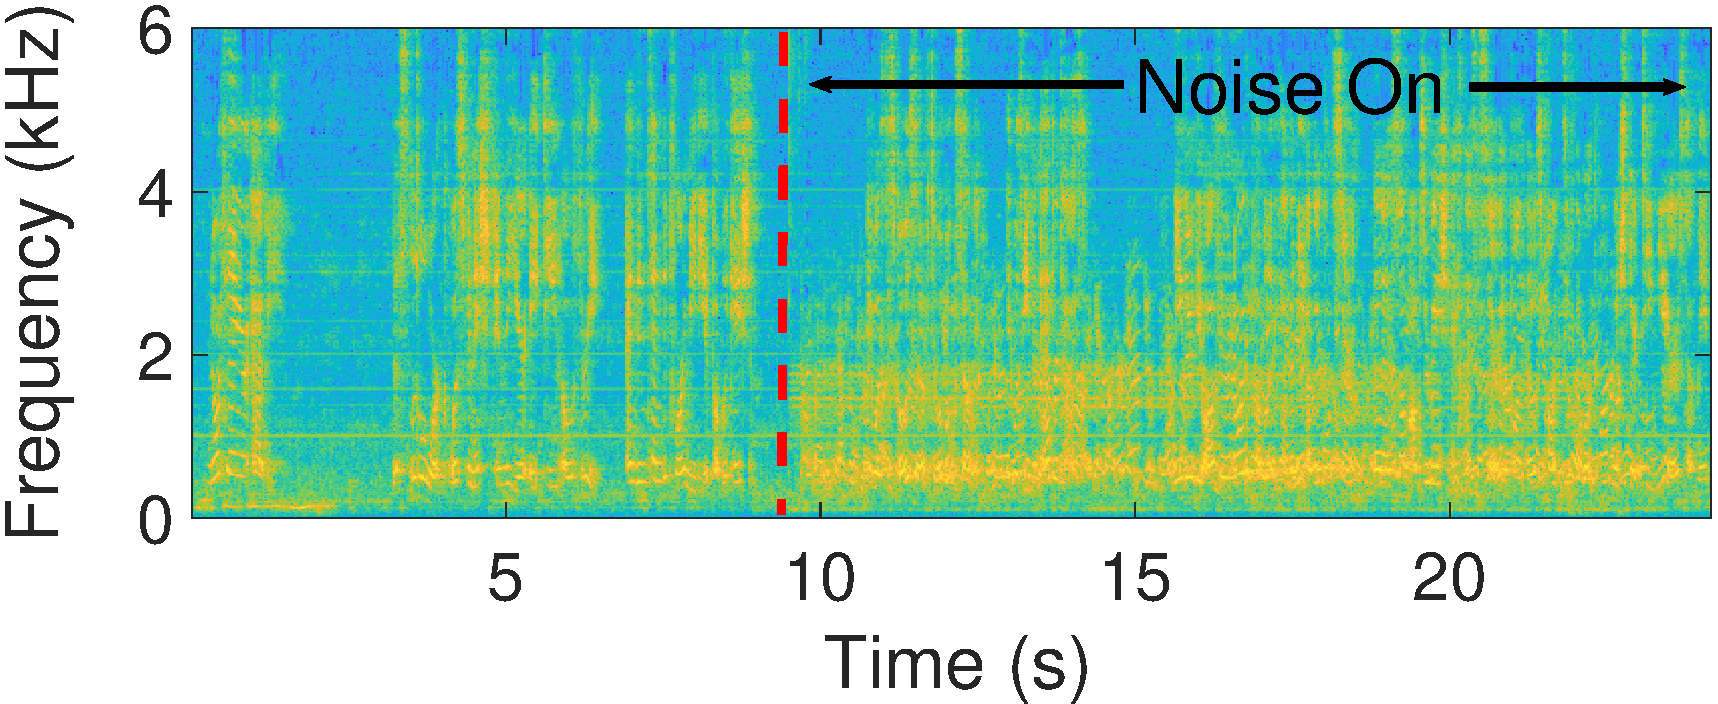
\includegraphics[width=\linewidth]{images/designed_denoise.pdf}
        \caption{Phoneme-Based Noise}    
        \label{fig:designed_denoise}
    \end{subfigure}
    \begin{subfigure}[b]{0.49\columnwidth}  
        \centering 
        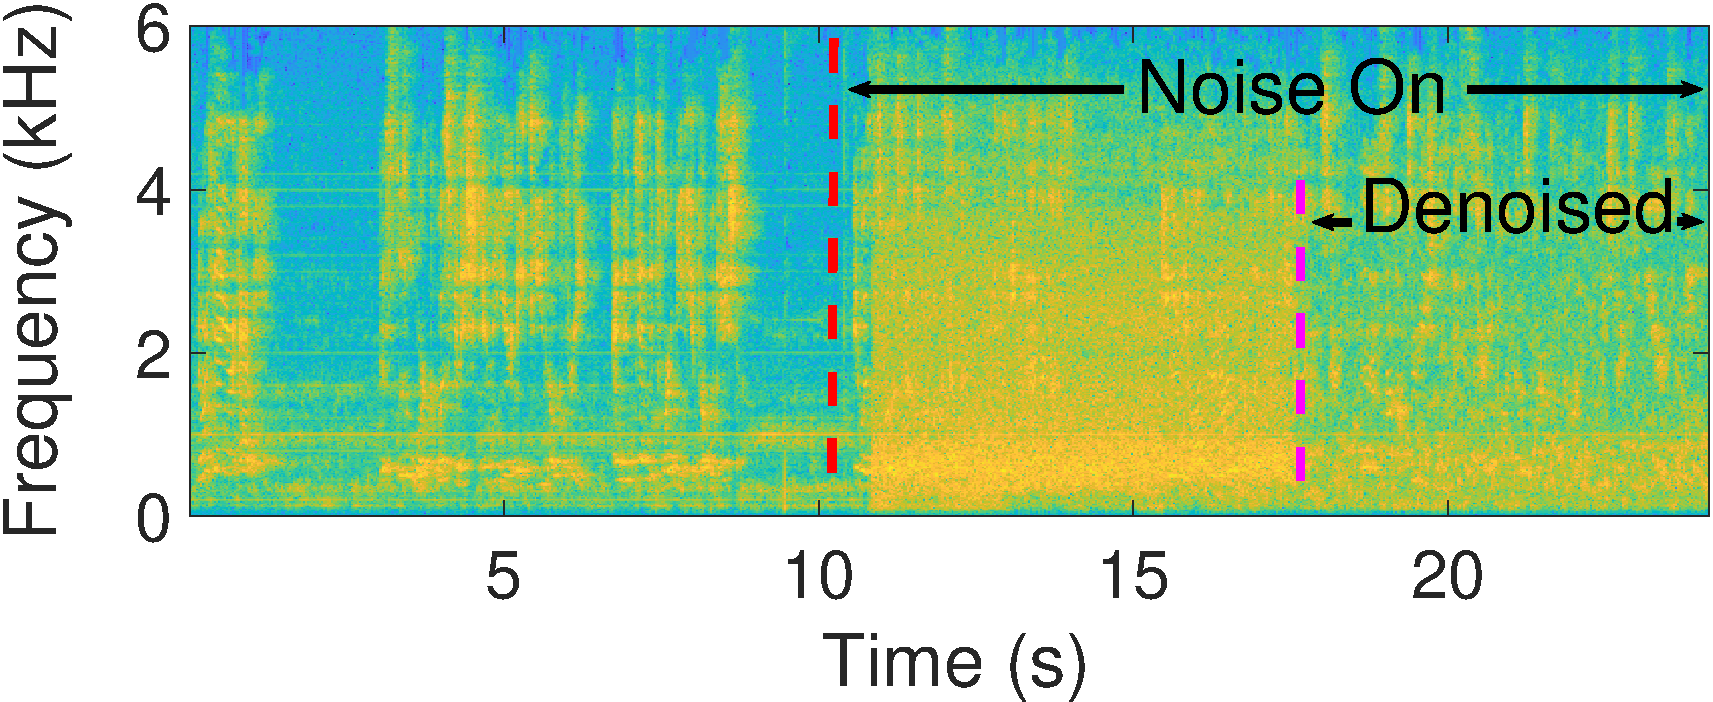
\includegraphics[width=\linewidth]{images/white_denoise.pdf}
        \caption{White Noise}    
        \label{fig:white_denoise}
    \end{subfigure}

    \begin{subfigure}[b]{0.49\columnwidth}   
        \centering 
        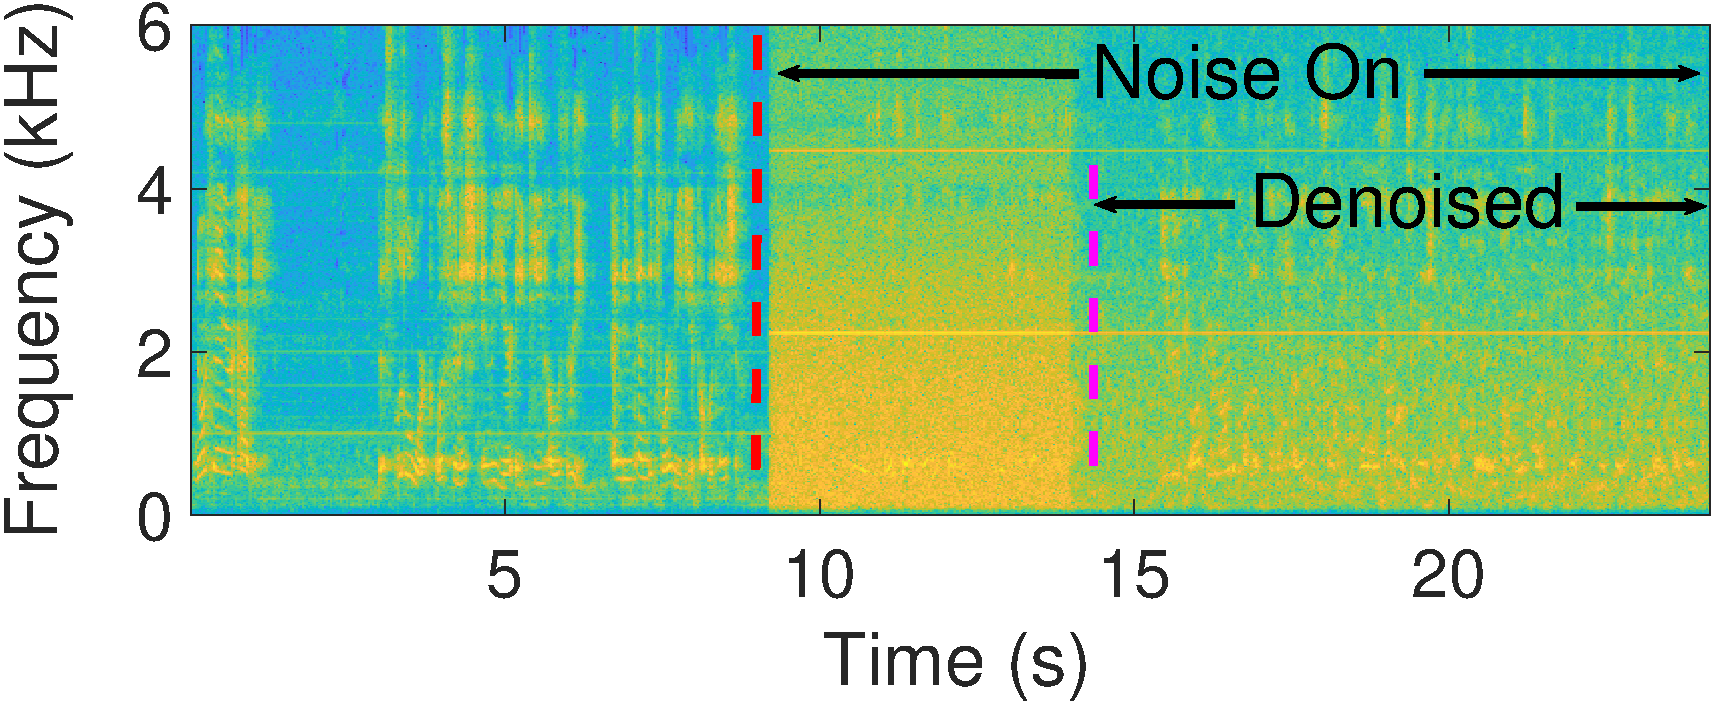
\includegraphics[width=\linewidth]{images/chi_denoise.pdf}
        \caption{Noise in \cite{CHI}}
        \label{fig:chi_denoise}
    \end{subfigure}
    \begin{subfigure}[b]{0.49\columnwidth}   
        \centering 
        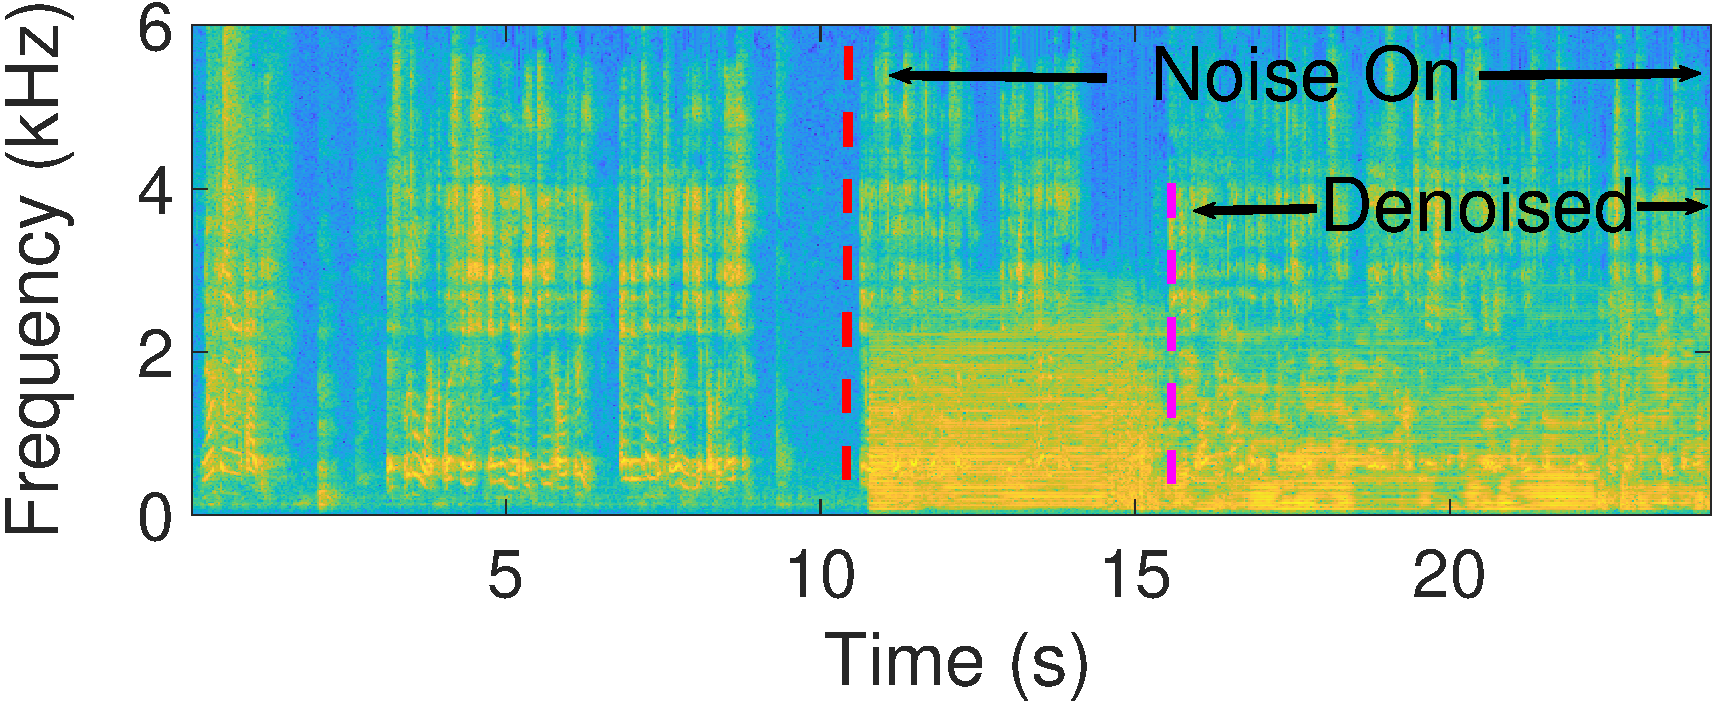
\includegraphics[width=\linewidth]{images/commercial_denoise.pdf}
        \caption{Noise Generated by \cite{commercial_device}}
        \label{fig:commercial_denoise}
    \end{subfigure}

    \caption{Comparison of robustness of different noises against the built-in noise reduction in a Vivo Nex smartphone.}
    \label{fig:test_denoise_in_noise_design}
    \vspace{-6mm}
\end{figure}